% change according to folder and file names
\ifpdf
    \graphicspath{{4/figures/PNG/}{4/figures/PDF/}{3/figures/}}
\else
    \graphicspath{{4/figures/EPS/}{4/figures/}}
\fi

%: ----------------------- contents from here ------------------------
\chapter{ΕΑ και ΜΑΕΑ για <<κακώς>> τοποθετημένα προβλήματα βελτιστοποίησης} % top level followed by section, subsection
\label{VarCorrChapter}
%\begin{flushright}
%Any intelligent fool can make things  
%\linebreak
%bigger, more complex, and more violent. 
%\linebreak
%It takes a touch of genius, and a lot of  
%\linebreak
%courage, to move in the opposite direction.
%\linebreak
%Albert Einstein
%\end{flushright}
Το κεφάλαιο αυτό έχει σκοπό να παρουσιάσει τρόπους με τους οποίους μπορεί να μειωθεί σημαντικά ο χρόνος βελτιστοποίησης με χρήση ΕΑ (ή  παραλλαγών αυτών και, μάλιστα, υπερθετικά στη μείωση που επιφέρουν διάφοροι άλλοι ήδη γνωστοί τρόποι, όπως λ.χ. η προσεγγιστική προ-αξιολόγηση με μεταπρότυπα, κτλ.) αν αναγνωρισθούν οι συσχετίσεις των μεταβλητών σχεδιασμού (ΣΜΣ) ως προς τη συνάρτηση κόστους $f$ \cite{Salomon,Roy_2002a,Ghisu_2010} στην υπόψη συνάρτηση κόστους και γίνει εκμετάλλευση της σχετικής πληροφορίας. Χωρίς βλάβη της γενικότητας, η παρουσίαση των προτεινόμενων τρόπων παρέμβασης στους ΕΑ ή τους ΜΑΕΑ θα γίνει για τη μονοκριτηριακή βελτιστοποίηση. Η γενίκευση, όμως, στην πολυκριτηριακή βελτιστοποίηση είναι προφανής. 

Οι συσχετίσεις των μεταβλητών σχεδιασμού ενός προβλήματος αναφέρονται πάντα ως προς την υπόψη συνάρτηση-κόστους $f$ και, προφανώς είναι συνυφασμένες άμεσα με την έννοια των ΣΜΣ είναι οι έννοιες της ισότροπης ή μη-ισότροπης επίδρασης των μεταβολών τιμής των μεταβλητών σχεδιασμού στη μεταβολή τιμής της $f$ και, κυρίως, του διαχωρίσιμου της. Η διαχείριση μιας μη-διαχορίσιμης, μη-ισότροπης συνάρτησης-στόχου $f$ κάνει το πρόβλημα βελτιστοποίησης <<κακώς-τοποθετημένο>> (\english{ill-posed}). Ειδικά τα μεγάλης διάστασης ($N>>$) κακώς-τοποθετημένα προβλήματα βελτιστοποίησης χαρακτηρίζονται από μεγάλο κόστος επίλυσης μέσω ΕΑ αλλά και ΜΑΕΑ. Επειδή δε τα περισσότερα βιομηχανικά προβλήματα ανήκουν σε αυτήν την κατηγορία, το ενδεχόμενο για μείωση του κόστους επίλυσής τους είναι τεράστιο.  Οι έννοιες της ισοτροπίας και του διαχωρίσιμου, καθώς και η επίδρασή τους στους ΕΑ, αναλύονται στην επόμενη ενότητα αυτού του κεφαλαίου. Από την άλλη πλευρά, από μαθηματικής σκοπιάς, ο εντοπισμός των ΣΜΣ υλοποιείται με την Ανάλυση σε Κύριες Συνιστώσες (ΑσΚΣ, \english{Principal Component Analysis \greek{ή} PCA}) \cite{Haykin}. Το κόστος χρήσης της ΑσΚΣ για τους σκοπούς του κεφαλαίου αυτού είναι το κόστος επίλυσης ιδιοπροβλημάτων μικρής διάστασης και είναι, ως εκ τούτου, πάρα πολύ μικρό. Γίνεται, μάλιστα, αμελητέο όταν ο ΕΑ ή ΜΑΕΑ χρησιμοποιεί υψηλού κόστους λογισμικό αξιολόγησης των υποψήφιων λύσεων, όπως λ.χ. κώδικες ΥΡΔ.

Το κεφάλαιο αυτό προτείνει και πιστοποιεί ως προς την αποδοτικότητα τους δύο τρόπους εκμετάλλευσης των ΣΜΣ (ως προς τη $f$) που εντοπίζει η ΑσΚΣ ή \english{PCA}. Ο πρώτος τρόπος σχετίζεται με την τροποποίηση των εξελικτικών τελεστών και θα αναφέρεται ως ΕΑ(\english{PCA}) ή ΜΑΕΑ(\english{PCA}) \cite{LTT_2_054}. Ο δεύτερος τρόπος σχετίζεται με τη χρήση μεταπροτύπων στο ΜΑΕΑ. Συγκεκριμένα, χρησιμοποιεί τις αναγνωρισθείσες ΣΜΣ κατά την ΠΠΑ των υποψήφιων λύσεων με μεταπρότυπα, ώστε τα τελευταία να εκπαιδεύονται με μικρό αριθμό σημαντικών εισόδων. Η μείωση αυτή του αριθμού εισόδων των μεταπροτύπων αυξάνει την αξιοπιστία τους, επιτρέπει τη χρήση τους νωρίτερα στο ΜΑΕΑ και οδηγεί σε υπολογιστικό κέρδος. Ο δεύτερος αυτός τρόπος θα αναφέρεται ως Μ(\english{PCA})ΑΕΑ. Στο ακρωνύμιο αυτό, ο προσδιορισμός \english{PCA} τοποθετείται μετά το Μ (Μ=\english{metamodel}, μεταπρότυπο) για να φανεί ακριβώς το που χρησιμοποιείται. Προφανώς, οι δύο τρόποι μπορούν να χρησιμοποιηθούν συνδυαστικά, οδηγώντας σε μέθοδο που θα αποκαλείται Μ(\english{PCA})ΑΕΑ(\english{PCA}).

Στο δεύτερο τμήμα του κεφαλαίου αυτού, οι προτεινόμενες τεχνικές δοκιμάζονται και πιστοποιούνται σε προβλήματα ελαχιστοποίησης κακώς-τοποθετημένων μαθηματικών συναρτήσεων. Στη συνέχεια, εκτίμηση του αναμενόμενου κέρδους γίνεται και σε ένα πρόβλημα σχεδιασμού-βελτιστοποίησης της μορφής της αεροτομής μιας 2Δ πτερύγωσης συμπιεστή. Βιομηχανικού ενδιαφέροντος εφαρμογές των προτεινόμενων μεθόδων παρουσιάζονται σε επόμενα κεφάλαια.             

 
%Σε αυτό το κεφάλαιο αρχικά παρουσιάζονται οι πιθανές ιδιαιτερότητες μιας συνάρτησης κόστους που ενδέχεται να προκαλέσουν συσχετίσεις μεταξύ των μεταβλητών σχεδιασμού (ΣΜΣ) \cite{Salomon,Roy_2002a,Ghisu_2010}. Στη συνέχεια, διερευνάται η επίδραση τους στους ΕΑ και αργότερα προτείνεται μία μέθοδος εντοπισμού αυτών των συσχετίσεων κάνονας χρήση Ανάλυσης σε Κύριες Συνιστώσες (ΑσΚΣ), \english{Principal Component Analysis (PCA)} και μέθοδοι αξιοποίησης τους αναβαθμίζοντας του τελεστές εξέλιξης. Προτείνεται, επίσης, η χρήση των ιδιοτιμών που υπολογίζονται από την ΑσΚΣ σαν μετρική σημαντικότητας των κατευθύνσεων στον χώρο σχεδιασμού και η αποκοπή των λιγότερο σημαντικών από αυτές κατά τη διαδικασία εκπαίδευσης του μεταπροτύπου.

%Τέλος οι προτεινόμενες τεχνικές πιστοποιούνται μέσα από αριθμό προβλημάτων μαθηματικής βελτιστοποίησης, ειδικά επιλεγμένων ούτως ώστε να εμπίπτουν στην κατηγορία των προβλημάτων με ΣΜΣ, και στον σχεδιασμό 2Δ πτερύγωσης συμπιεστή.
    
\section{Δυσκολίες λόγω ιδιαιτερότητας της συνάρτησης κόστους}
Ένα πρόβλημα βελτιστοποίησης αναφέρεται ως <<κακώς τοποθετημένο>> αν παρουσιάζει συνδυασμό δύο ιδιαιτεροτήτων της συνάρτησης-κόστους $f$ (σχήμα \ref{nonsep}): α) τη μη-ισότροπη συνεισφορά των μεταβλητών σχεδιασμού στη συνάρτηση κόστους και β) το μη-διαχωρίσιμο της $f$.

Μη-ισότροπη συνεισφορά των μεταβλητών σχεδιασμού στη συνάρτηση-κόστους υπάρχει όταν ισόποσες μεταβολές των μεταβλητών σχεδιασμού δεν επιφέρουν ισόποσες μεταβολές στην τιμή της $f$.  Μια συνάρτηση-κόστους $f$ ονομάζεται διαχωρίσιμη ως προς τη μεταβλητή σχεδιασμού $x_i$ αν η βέλτιστη τιμή του $x_i$ είναι ανεξάρτητη των τιμών των υπολοίπων μεταβλητών σχεδιασμού. Η $f$ ονομάζεται διαχωρίσιμη αν είναι διαχωρίσιμη ως προς όλες τις μεταβλητές σχεδιασμού.        

\begin{figure}[h!]
\begin{minipage}[b]{1\linewidth}
 \centering
 \resizebox*{14cm}{!}{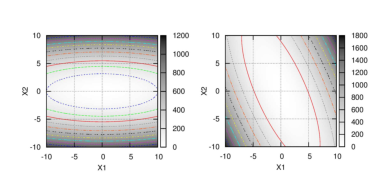
\includegraphics{ellipseB.eps}}
\end{minipage}
%\begin{minipage}[b]{0.45\linewidth}
% \centering
% \resizebox*{9cm}{!}{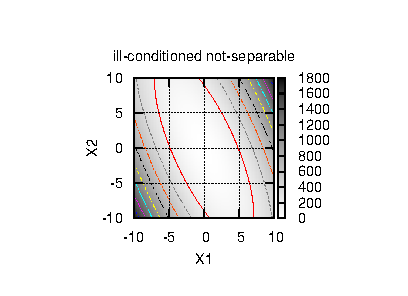
\includegraphics{ellipseturn.eps}}
%\end{minipage}
\caption{Πρόβλημα βελτιστοποίησης με μη-ισότροπη συνεισφορά των μεταβλητών σχεδιασμού στην $f$ (αριστερά). Πρόκειται για ισοϋψείς της $f$ της σχέσης \ref{ellipse} για Ν=2. Η μεταβλητή $x_2$ συνεισφέρει σε μεγαλύτερο βαθμό στην $f$ από ότι η $x_1$. Από την άλλη πλευρά, η $f$ είναι διαχωρίσιμη άρα το πρόβλημα, ουσιαστικά δεν είναι <<κακώς τοποθετημένο>>. Πρόβλημα βελτιστοποίησης με μη-ισότροπη συνεισφορά των μεταβλητών σχεδιασμού και μη-διαχωρίσιμες μεταβλητές σχεδιασμού ως προς την $f$ (δεξιά). Πρόκειται για ισοϋψείς της $f$ της σχέσης \ref{ellipse2} για Ν=2. Η βέλτιστη τιμή της $x_1$ εξαρτάται πλέον από τη $x_2$ και αντίστροφα. Άρα το πρόβλημα βελτιστοποίησης είναι πλέον <<κακώς τοποθετημένο>>, κάτι που θα φανεί ιδιαίτερα για μεγάλες τιμές του Ν.} 
\label{nonsep}
\end{figure}

Η επίδραση των παραπάνω χαρακτηριστικών στη συνάρτηση-στόχου $f$ σε ένα πρόβλημα βελτιστοποίησης, όταν αυτό επιλύεται με ΕΑ,  διερευνάται μέσω δύο προβλημάτων μαθηματικής βελτιστοποίησης επιλεγμένων ώστε να εμπίπτουν σε αυτήν την κατηγορία. Σκοπός της διερεύνησης είναι να δειχθεί ότι, αν το ίδιο πρόβλημα βελτιστοποίησης επαναδιατυπωθεί ως προς νέες μεταβλητές σχεδιασμού, ίδιου πλήθους, ως προς τις οποίες η υπόψη συνάρτηση κόστους είναι διαχωρίσιμη, ο ΕΑ εντοπίζει τη βέλτιστη λύση σε πολύ μικρότερο αριθμό αξιολογήσεων.  

Το πρώτο πρόβλημα αφορά ελαχιστοποίηση ενός πολυδιάστατου ελλειψοειδούς (η 2Δ μορφή του παρουσιάζεται στο σχήμα \ref{nonsep}). Η διαχωρίσιμη μορφή του περιγράφεται από τη σχέση   

\begin{eqnarray}
   f(\vec{x})=\sum^{N}_{i=1}a^{\frac{i-1}{N-1}}x_i^2
   \label{ellipse} 
\end{eqnarray}
όπου $a$ ο αριθμός κατάστασης της συνάρτησης. Μεγάλες τιμές της ποσότητας $a$ $(a>>1)$ ενισχύουν τη μη-ισότροπη συνεισφορά των μεταβλητών σχεδιασμού στην $f$.

Εναλλακτικά, μια μη-διαχωρίσιμη μορφή του ίδιου προβλήματος μπορεί να διατυπωθεί ως 
\begin{eqnarray}
   f(\vec{x})=\sum^{N}_{i=1}a^{\frac{i-1}{N-1}}y_i^2
   \label{ellipse2} 
\end{eqnarray}
όπου $\vec{y}=B\vec{x}$ και $B$ ένα ($N\times N$) μητρώο στροφής. Η σύγκριση των σχέσεων \ref{ellipse} και \ref{ellipse2} φαίνεται εποπτικά, για Ν=2, στο σχήμα \ref{nonsep}. Ουσιαστικά, οι σχέσεις \ref{ellipse} και \ref{ellipse2} αναφέρονται στο ίδιο πρόβλημα ελαχιστοποίησης, με τη μορφή \ref{ellipse} να πλεονεκτεί της \ref{ellipse2} όταν η επίλυση γίνεται μαι ΕΑ ή ΜΑΕΑ.  

Η δεύτερη περίπτωση μαθηματικής βελτιστοποίησης αφορά την ελαχιστοποίηση της πολυτροπικής συνάρτησης 

\begin{eqnarray}
   f(\vec{x})=10N+(\sum^{N}_{i=1}x_i)^2 - 10Ncos(\pi  \sum^{N}_{i=1}x_i)
   \label{mm} 
\end{eqnarray}

Η συνάρτηση \ref{mm} αποτελεί τη μη-διαχωρίσιμη εκδοχή του προβλήματος βελτιστοποίησης. Η αντίστοιχη διαχωρίσιμη εκδοχή υπάρχει και προκύπτει, όμοια με την περίπτωση του ελλειψοειδούς, αν το $\vec{x}$ αντικατασταθεί απο το $\vec{y}$ όπου $\vec{y}=B\vec{x}$ και $B$ κατάλληλο μητρώο στροφής. Η συνάρτηση \ref{mm}, έχοντας, στην πραγματικότητα, μόνο μια σημαντική κατεύθυνση στο χώρο σχεδιασμού, ανήκει στην κατηγορία των συναρτήσεων με εξαιρετικά μη-ισότροπη συνεισφορά των μεταβλητών σχεδιασμού στην $f$ ( ως εάν $a=\infty$). 
%Αυτή είναι μια πολύ σημαντική κατηγορία προβλημάτων γιατί προσομοιάζει σε συμπεριφορά τα προβλήματα βελτιστοποίησης πολλών στόχων, όπου στην πραγματικότητα μια περιοχή του χώρου των λύσεων εμπεριέχει όλους τους βέλτιστους σχεδιασμούς.           

Συγκριτικές πορείες σύγκλισης μεταξύ διαχωρίσιμης και μη-διαχωρίσιμης εκδοχής του $30$Δ ($N\!=\!30$) ελλειψοειδούς και της πολυτροπικής συνάρτησης \ref{mm} παρουσιάζονται στο σχήμα \ref{ellipse_t2}. Οι πορείες σύγκλισης απεικονίζουν μέσες τιμές υπολογισμένες για $10$ διαδικασίες βελτιστοποίησης ($10$ διαφορετικά τρεξίματα ΕΑ) με διαφορετική αρχικοποίηση της γεννήτριας τυχαίων αριθμών.  Παρατηρείται ότι και στις δύο περιπτώσεις η διαχωρίσιμη εκδοχή των προβλημάτων βελτιστοποίησης υπερτερεί σημαντικά σε ταχύτητα της μη-διαχωρίσιμης εκδοχής αυτών. Το κέρδος δε είναι σημαντικά μεγαλύτερο στην περίπτωση της όπου $a=\infty$.        

\begin{figure}[h!]
%\begin{minipage}[b]{0.5\linewidth}
% \centering
% \resizebox*{7.5cm}{!}{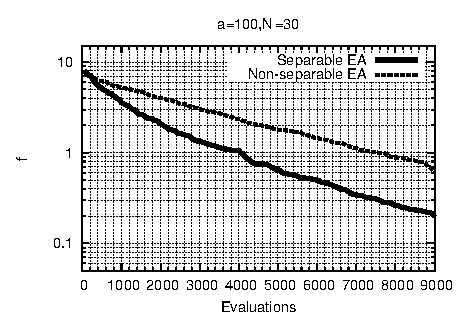
\includegraphics{100_30d.eps}}
%\end{minipage}
\begin{minipage}[b]{0.5\linewidth}
 \centering
 \resizebox*{7.5cm}{!}{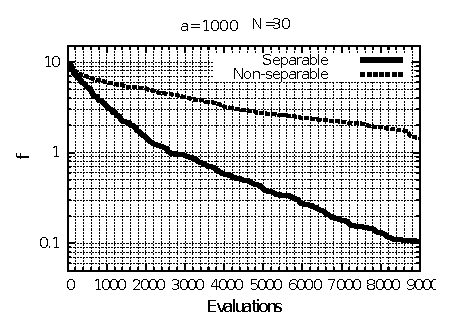
\includegraphics{1000_30db.eps}}
\end{minipage}
\begin{minipage}[b]{0.5\linewidth}
 \centering
 \resizebox*{7.5cm}{!}{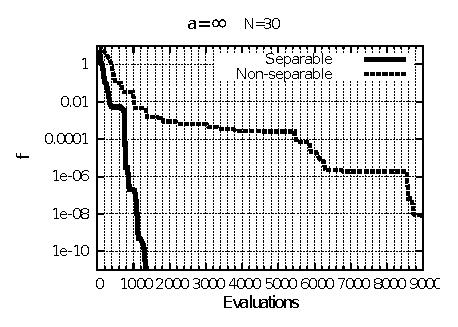
\includegraphics{30db.eps}}
\end{minipage}
\caption{Πορείες σύγκλισης ΕΑ για το 30Δ ελλειψοειδές με αριθμό κατάστασης (με $a=1000$) (αριστερά) και για την 30Δ συνάρτηση της σχέσης \ref{mm} ($a=\infty$)(δεξιά). Κάθε πρόβλημα λύνεται 10 φορές στη διαχωρίσιμη και άλλες 10 στη μη-διαχωρίσιμη εκδοχή του και σχεδιάζεται η μέση πορεία σύγκλισης κάθε περίπτωσης.} 
\label{ellipse_t2}
\end{figure}



\section{Υπολογισμός ΣΜΣ}
Η προτεινόμενη μέθοδος εντοπισμού των ΣΜΣ κάνει χρήση της ΑσΚΣ για να υπολογίσει τα τοπολογικά χαρακτηριστικά του συνόλου των επιλέκτων τα οποία και θεωρούνται αντιπροσωπευτικά των ΣΜΣ. Πιο αναλυτικά, αφού το σύνολο των επιλέκτων μετατραπεί σε ένα τυποποιημένο σύνολο δεδομένων Χ, \english{standardized data-set}, \cite{Axler_1997}, δημιουργείται ο πίνακας συνδιακύμανσης, \english{empirical covariance matrix
},  $P_{N\times N}$ από τη σχέση 

\begin{equation} 
   P_{N\times N}= \frac{1}{e}XX^T
   \label{Cov_Mat} 
\end{equation}
όπου $e$ το μέγεθος του συνόλου των επίλεκτων $P_e^g$ και $X$ ο πίνακας που έχει σαν γραμμές τα διανύσματα σχεδιασμού των μελών του $P_e^g$ σε μορφή τυποποιημένου συνόλου δεδομένων.

Κάνοντας χρήση του φασματικού θεωρήματος αποσύνθεσης (\english{spectral decomposition theorem})
 \cite{Axler_1997, Fodor_2002}, ο $P_{N\times N}$ μπορεί να γραφεί ως

\begin{equation} 
   P_{N\times N}= U\Lambda U^T
   \label{spectral}
\end{equation}
όπου $\Lambda\!=\!diag(\lambda_1 , . . . , \lambda_N )$ το διαγώνιο μητρώο των ιδιοτιμών και $U$ το $N\!\times\!N$ μητρώο των ιδιοδιανύσματων. 
Τα υπολογισθέντα ιδιοδιανύσματα (σχήμα \ref{reco1}) είναι οι κατευθύνσεις, στο χώρο σχεδιασμού, ως προς τις οποίες η $f$ είναι, κατά το δυνατό, διαχωρίσιμη. Αν ο ΕΑ χειριζόταν αυτές τις κατευθύνσεις, το πρόβλημα βελτιστοποίησης θα μετατρέπονταν σε, κατά το δυνατό, διαχωρίσιμο και άρα θα επιλύονταν με μικρότερο υπολογιστικό κόστος.    

\begin{figure}[h!]
\begin{minipage}[b]{1\linewidth}
 \centering
 \resizebox*{!}{4.5 cm}{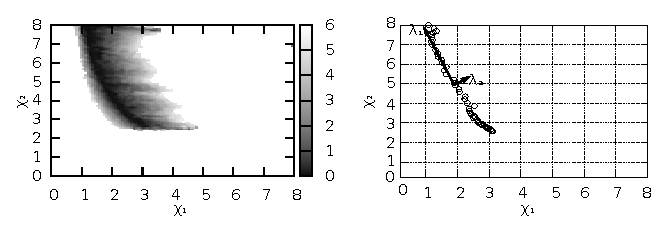
\includegraphics{DOFs.eps}}
\end{minipage}
\caption{Κατανομή της $f$ (ή της βαθμωτής $\Phi$ από λ.χ. τη διαδικασία \english{SPEA2}, για κάποια γενιά κατά την εξέλιξη, σε προβλήματα πολυκριτηριακής βελτιστοποίησης) στο χώρο σχεδιασμού (αριστερά). Το σύνολο των επίλεκτων $P^g_e$, για τη δεδομένη γενιά, και οι οι κατευθύνσεις, στον χώρο σχεδιασμού, που υποδηλώνουν τις ΣΜΣ $\lambda_1$ και $lambda_2$ (αριστερά).} 
\label{reco1}
\end{figure}
       

\section{Εξελικτικοί τελεστές υποβοηθούμενοι από ΑσΚΣ} 

Με στόχο την επαναδιατύπωση του προβλήματος βελτιστοποίησης, μετά την αναγνώριση των ΣΜΣ για την υπόψη $f$ η παρούσα διατριβή προτείνει την εφαρμογή των τελεστών εξέλιξης (μετάλλαξης και διασταύρωσης), στο ευθυγραμμισμένο με τις νέες μη-συσχετιζόμενες μεταβλητές σχεδιασμού που ανέδειξε η ΑσΚΣ. Με αυτήν την τακτική, η εξέλιξη λαμβάνει χώρα στο μετασχηματισμένο και κατά το δυνατό διαχωρίσιμο πρόβλημα βελτιστοποίησης, έχοντας σκοπό να ανακτήσει το μεγαλύτερο δυνατό ποσοστό απώλειας αποδοτικότητας του ΕΑ (σχήμα \ref{ellipse_t2}), που προκαλεί το μη-διαχωρισμό της $f$. Πληροφορίες σχετικές με τις ΣΜΣ προσδιορίζονται εκ νέου μέσω της ΑσΚΣ, κάθε φορά που ένα νέο άτομο προστίθεται στο σύνολο των επιλέκτων και η ποιότητα τους αυξάνεται όσο το σύνολο των επιλέκτων προσεγγίζει το πραγματικό μέτωπο \english{Pareto}.              

%\begin{figure}[h!]
%\begin{minipage}[b]{1\linewidth}
% \centering
% \resizebox*{14cm}{!}{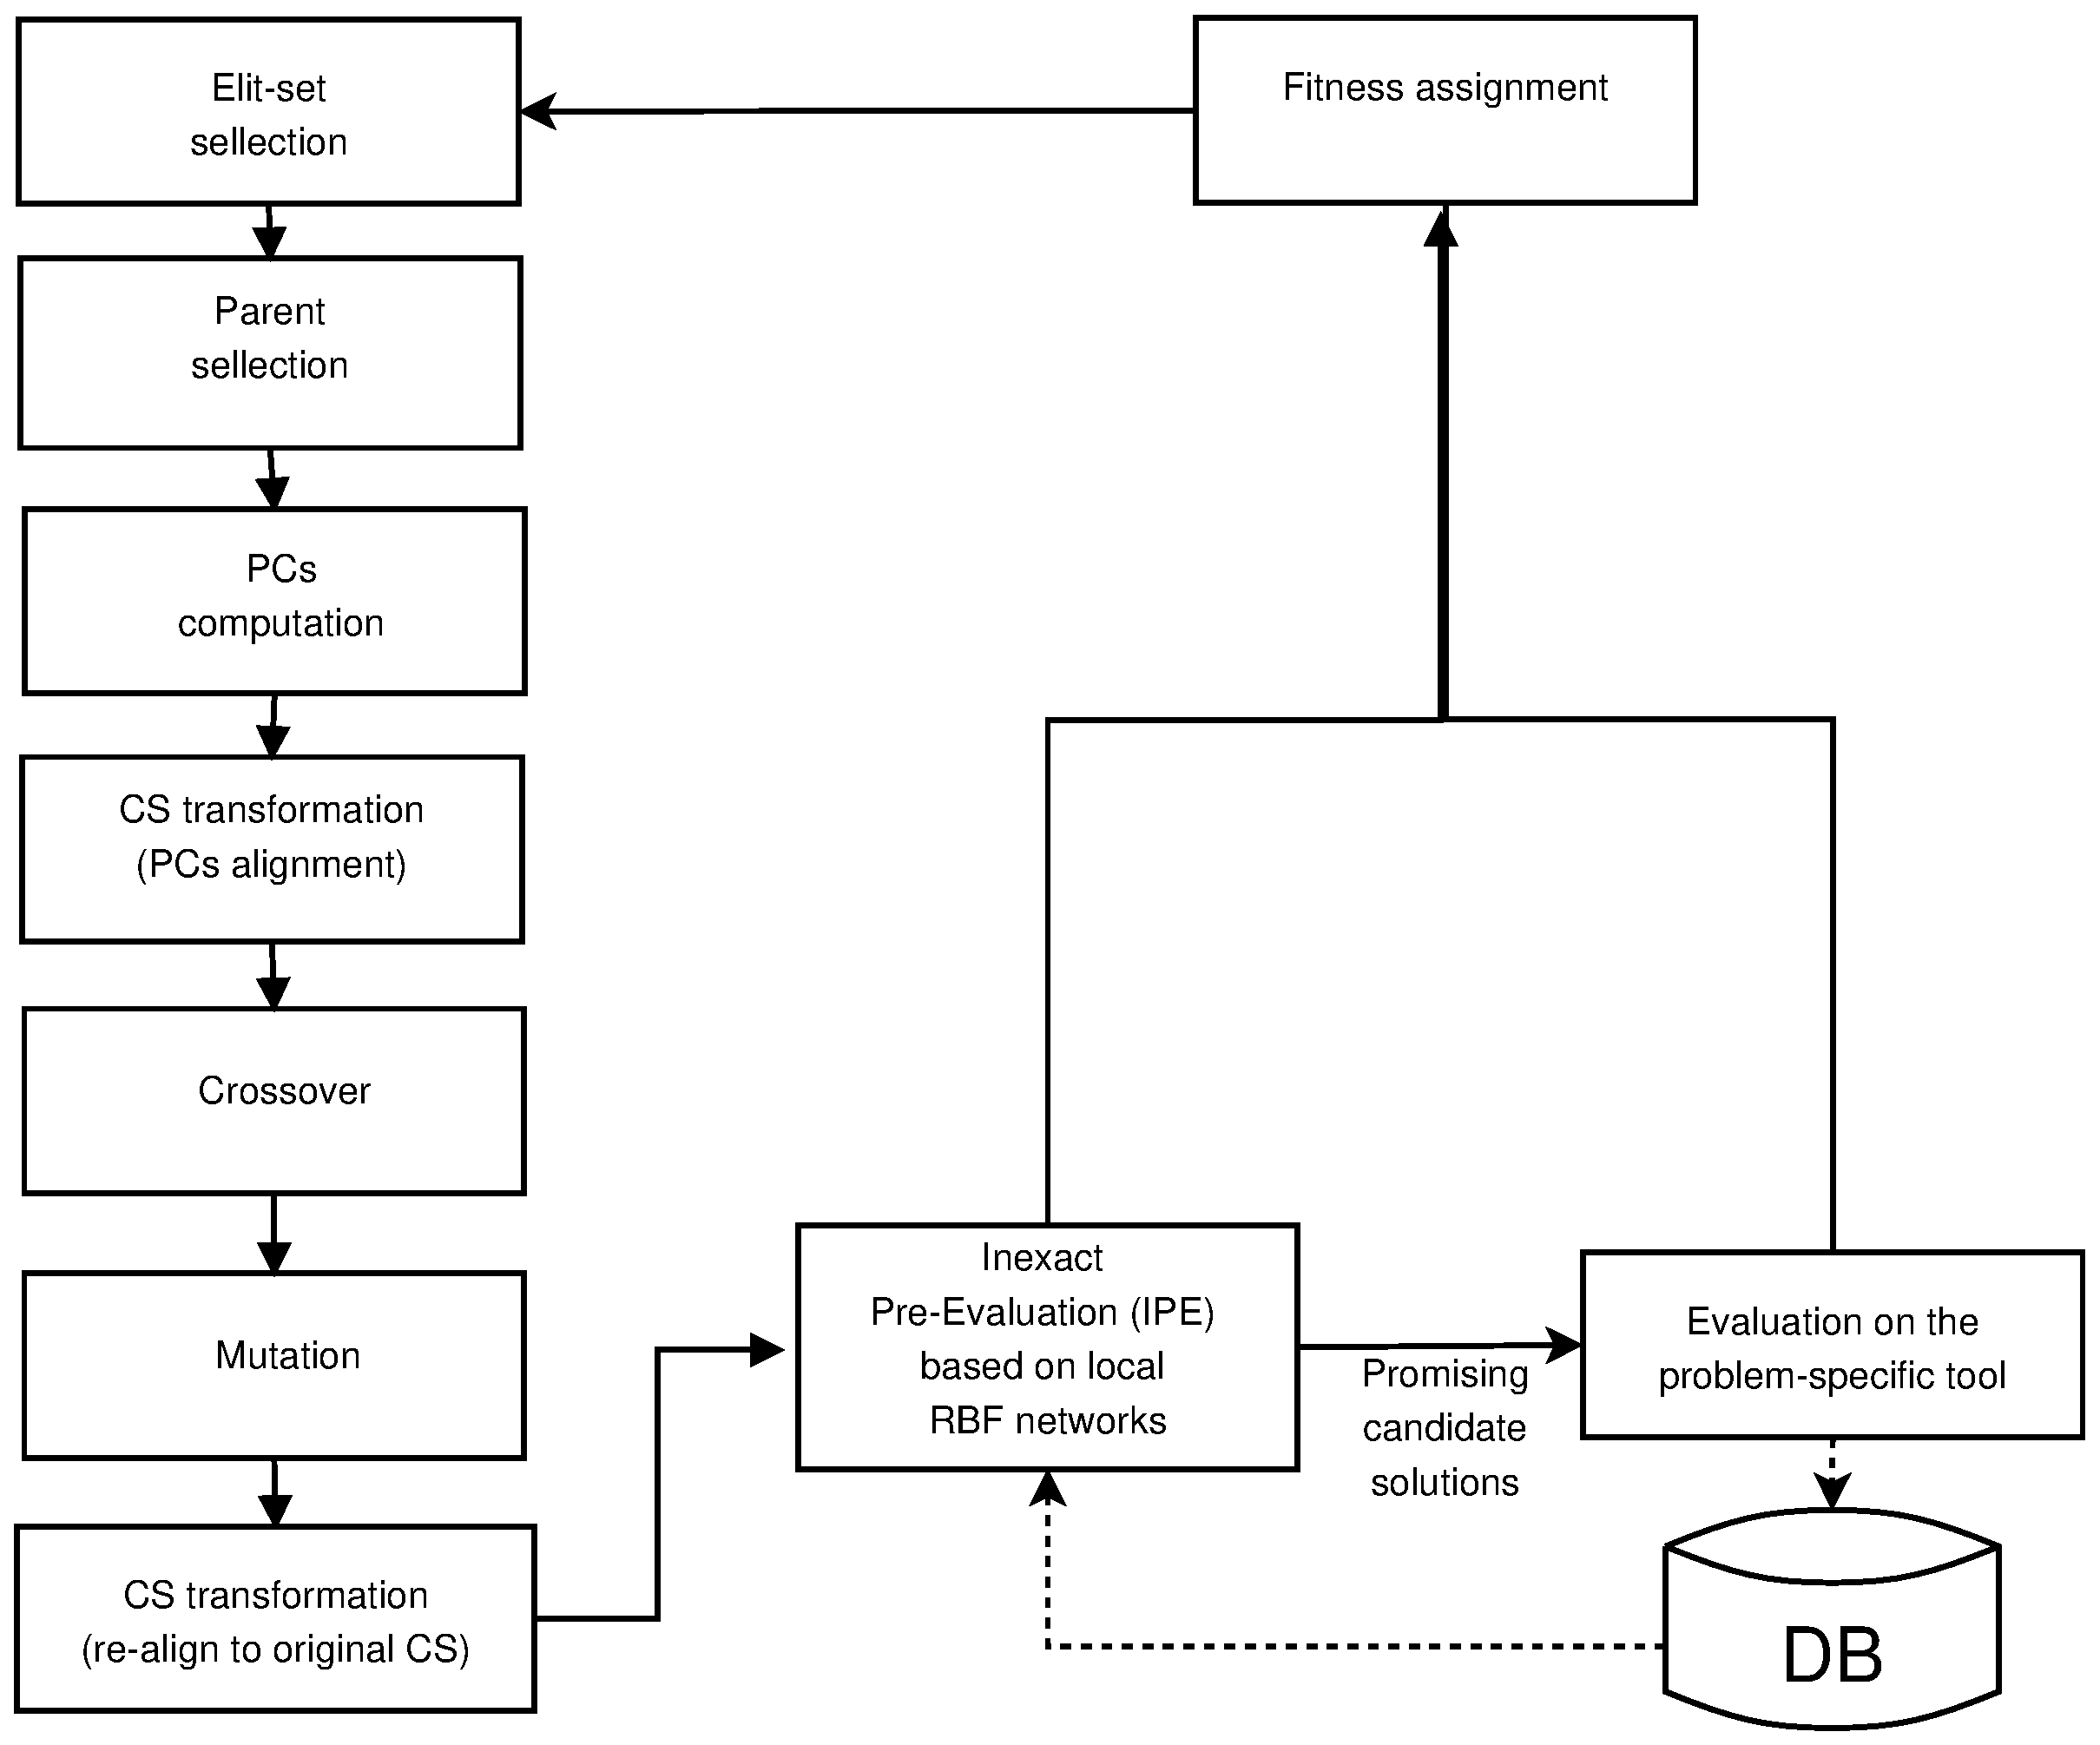
\includegraphics{MAEAPCA2.eps}}
%\end{minipage}
%\caption{Σχηματική απεικόνιση υποβοηθούμενου από μεταπρότυπα ΕΑ που κάνει χρίση τελεστών εξέλιξης υποβοηθούμενων από ΑσΚΣ (\english{MAEA(PCA)}).} 
%\label{MAEAPCA2}
%\end{figure}

\subsection{Πιστοποίηση εξελικτικών τελεστών υποβοηθούμενων από ΑσΚΣ}
Το κέρδος απο τη χρήση των εξελικτικών τελεστών στις μη - συσχετιζόμενες μεταβλητές σχεδιασμού που ανέδειξε η ΑσΚΣ  ποσοτικοποιείται στα προβλήματα μαθηματικής ελαχιστοποίησης του 30Δ ελλειψοειδούς (σχέση \ref{ellipse}) και τις 30Δ πολυτροπικής συνάρτησης (σχέση \ref{mm}). 



\begin{figure}[h!]
%\begin{minipage}[b]{0.5\linewidth}
% \centering
% \resizebox*{7.5cm}{!}{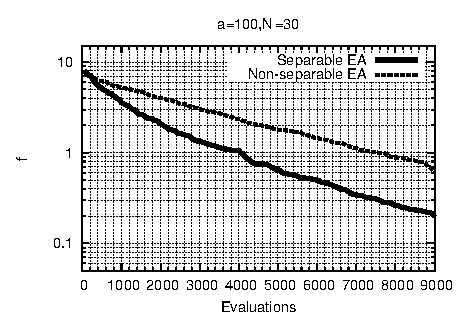
\includegraphics{100_30d.eps}}
%\end{minipage}
\begin{minipage}[b]{0.5\linewidth}
 \centering
 \resizebox*{7.5cm}{!}{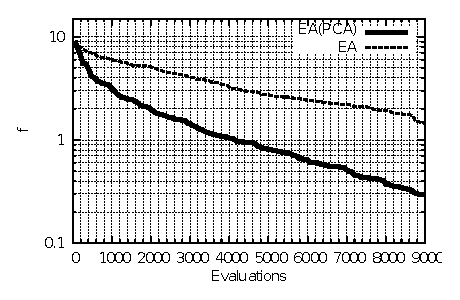
\includegraphics{1000_30d_pca.eps}}
\end{minipage}
\begin{minipage}[b]{0.5\linewidth}
 \centering
 \resizebox*{7.5cm}{!}{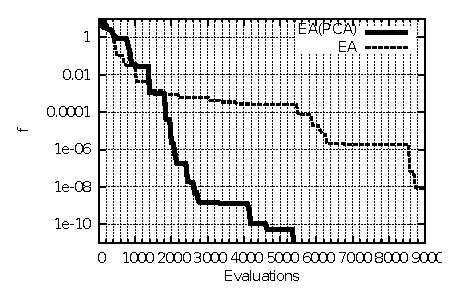
\includegraphics{30d_pca.eps}}
\end{minipage}
\caption{Πορείες σύγκλισης για το 30Δ ελλειψοειδές με αριθμό κατάστασης ($a\!=\!1000$) (αριστερά)  και για την 30Δ συνάρτηση \ref{mm} (δεξιά). Η έντονη γραμμή παρουσιάζει την κατά πολύ βελτιωμένη σύγκλιση του ΕΑ στον οποίο οι εξελικτικοί τελεστές εφαρμόστηκαν στις εντοπιζόμενες από ΑσΚΣ διαχωρίσημες μεταβλητές σχεδιασμού.} 
\label{ellipse_t2_pca}
\end{figure} 

Οι πορείες σύγκλισης των ΕΑ και ΕΑ(\english{PCA}) για το $30$Δ ελλειψοειδές και την πολυτροπική συνάρτηση \ref{mm} παρουσιάζονται στο σχήμα \ref{ellipse_t2_pca}. Οι καμπύλες που σχεδιάζονται αποτελούνται, και πάλι, από τις μέσες τιμές των πορειών σύγκλισης που υπολογίσθηκαν τρέχοντας το ίδιο πρόβλημα $10$ φορές, κάθε φορά με διαφορετική αρχικοποίηση της γεννήτριας τυχαίων αριθμών.  Παρατηρείται ότι, και στα δύο προβλήματα, η χρήση των υποβοηθούμενων από την ΑσΚΣ τελεστών εξέλιξης υπερτερεί σημαντικά σε ταχύτητα και ανακτά ένα σημαντικό μέρος της μειωμένης αποδοτικότητας των ΕΑ όταν αυτοί χρησιμοποιούνται για να λύσουν <<κακώς τοποθετημένα>> προβλήματα βελτιστοποίησης. 


\section{Μεταπρότυπα υποβοηθούμενα από ΑσΚΣ}
Η χρήση της ΑσΚΣ κατά τη διάρκεια εφαρμογής των τελεστών εξέλιξης δεν είναι η μόνη τεχνική που προτάθηκε και αποδείχθηκε ιδιαίτερα αποδοτική. Στην παρούσα διατριβή, επιπροσθέτως προτείνεται και η χρήση των υπολογισθέντων, κατά την ΑσΚΣ, ιδιοτιμών ως μετρικών σημαντικότητας των κατευθύνσεων στο χώρο σχεδιασμού. Με τον τρόπο αυτό, η εκπαίδευση των μεταπροτύπων ενός ΜΑΕΑ πραγματοποιείται σε χώρο με αισθητά μειωμένη διάσταση. Τα μεταπρότυπα εκπαιδεύονται με μειωμένο αριθμό εισόδων, συγκρατώντας και χρησιμοποιώντας μόνο τις σημαντικότερες κατευθύνσεις στο χώρο σχεδιασμού που ανέδειξε η ΑσΚΣ και αποκόπτοντας τις λιγότερο σημαντικές. Η σημαντικότητα ορίζεται ως αντιστρόφως ανάλογη της ιδιοτιμής κάθε κατεύθυνσης στο χώρο σχεδιασμού (σχήμα \ref{1dann}).              

\begin{figure}[h!]
\begin{minipage}[b]{0.5\linewidth}
 \centering
 \resizebox*{7.0cm}{!}{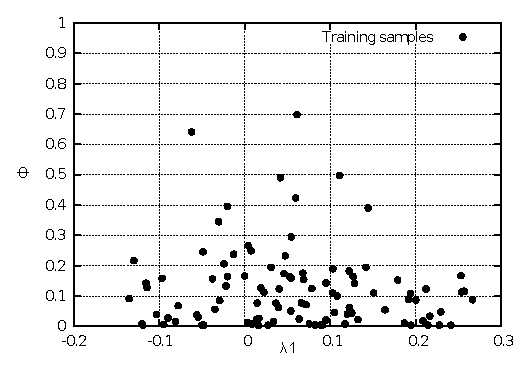
\includegraphics{1dANN_e1.eps}}
\end{minipage}
\begin{minipage}[b]{0.5\linewidth}
 \centering
 \resizebox*{7.0cm}{!}{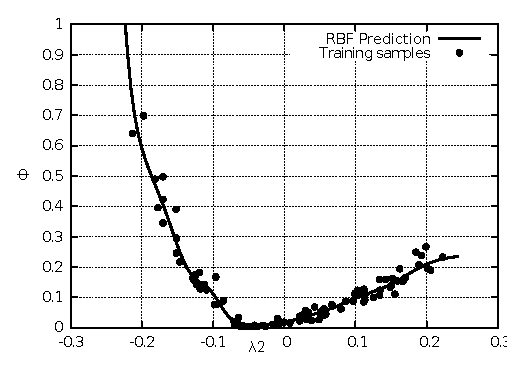
\includegraphics{1dANN_e2.eps}}
\end{minipage}
\caption{Εκτιμήσεις της τιμής της $\Phi$ από το μεταπρότυπο στο 2Δ πρόβλημα βελτιστοποίησης του σχήματος \ref{reco1}.  Πρότυπα εκπαίδευσης προβεβλημένα στο επίπεδο ($\Phi,\lambda_1$), όπου $\lambda_1$ η κατεύθυνση με τη μεγάλη ιδιοτιμή, βάσει της πραγματοποιηθείσας ΑσΚΣ (αριστερά). Πρότυπα εκπαίδευσης προβεβλημένα στο επίπεδο ($\Phi,\lambda_2$), όπου $\lambda_2$ η κατεύθυνση με τη μικρή ιδιοτιμή (δεξιά). Στην παρούσα διατριβή προτείνεται το μεταπρότυπo να εκπαιδευτεί μόνο στο  ($\Phi,\lambda_2$) επίπεδο, με το $\lambda_2$ δηλαδή ως τη μοναδική του είσοδο. Στο δεξιό σχήμα, με συνεχή γραμμή σχεδιάζεται η αναμενόμενη πρόβλεψη από το «σωστά» εκπαιδευμένο δίκτυο \english{RBF}. Στο αριστερό σχήμα, η αντίστοιχη καμπύλη αδυνατεί να παρακολουθήσει την ακατάστατη μορφή μορφή των αποκρίσεων και, για το λόγο αυτό, δεν σχεδιάζεται.} 
\label{1dann}
\end{figure}

Είναι εμφανές το πλεονέκτημα που επιφέρει η εκπαίδευση ενός μεταπροτύπου μόνο με τη συνιστώσα $\lambda_2$ (σχήμα \ref{1dann}), μιας και η κατά $\lambda_1$ συνιστώσα εισάγει ανεπιθύμητο θόρυβο και κάνει λιγότερο αξιόπιστη τη πρόβλεψη της $\Phi$ από το μεταπρότυπο.   

\subsection{Πιστοποίηση του Μ($PCA$)ΑΕΑ($PCA$)}

Η επιπλέον χρήση των προτεινόμενων, υποβοηθούμενων από ΑσΚΣ, μεταπροτύπων, δηλαδή η τεχνική Μ(\english{PCA})ΑΕΑ(\english{PCA}), πιστοποιείται στα προβλήματα ελαχιστοποίησης του 30Δ ελλειψοειδούς (σχέση \ref{ellipse}) και της 30Δ πολυτροπικής συνάρτησης (σχέση \ref{mm}). 


\begin{figure}[h!]
\begin{minipage}[b]{0.5\linewidth}
 \centering
 \resizebox*{7.5cm}{!}{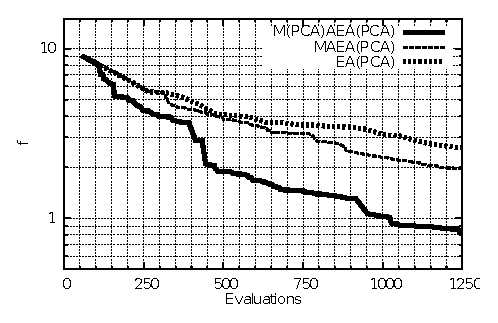
\includegraphics{1000_30d_pca_ipe.eps}}
\end{minipage}
\begin{minipage}[b]{0.5\linewidth}
 \centering
 \resizebox*{7.5cm}{!}{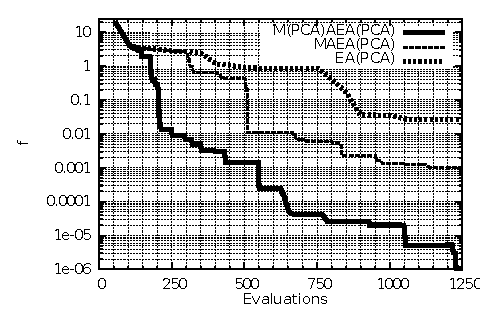
\includegraphics{30d_pca_ipe.eps}}
\end{minipage}
\caption{Μέσες καμπύλες σύγκλισης παραλλαγών των ΕΑ ή ΜΑΕΑ, που χρησιμοποιούν ΑσΚΣ, για το 30Δ ελλειψοειδές με  αριθμό κατάστασης $a=1000$ (αριστερά), και για την 30Δ συνάρτηση της σχέσης \ref{mm} (δεξιά).} 
\label{ellipse_t2_pca_ipe}
\end{figure} 

Οι πορείες σύγκλισης των ΕΑ(\english{PCA}),    ΜΑΕΑ(\english{PCA}) και \linebreak Μ(\english{PCA})ΑΕΑ(\english{PCA}) για τα δύο αυτά προβλήματα παρουσιάζονται στο σχήμα \ref{ellipse_t2_pca_ipe}. Οι πορείες σύγκλισης αποτελούνται από μέσες τιμές υπολογισμένες για $10$ διαδικασίες βελτιστοποίησης με διαφορετική αρχικοποίηση της γεννήτριες τυχαίων αριθμών.  Παρατηρείται ότι η επιπρόσθετη χρήση υποβοηθούμενων απο ΑσΚΣ μεταπροτύπων επιφέρει επιπλέον μείωση του υπολογιστικού κόστους και για τις δύο περιπτώσεις.


\section{Εφαρμογή: Σχεδιασμός 2Δ πτερύγωσης συμπιεστή}
Οι προτεινόμενες σε αυτό το κεφάλαιο μέθοδοι πιστοποιούνται, επίσης, στο σχεδιασμό-βελτιστοποίηση της αεροτομής μιας 2Δ πτερύγωσης συμπιεστή. Η πτερύγωση λειτουργεί σε $M_1=0.54$, $a_1=44^o$ και $Re=4\!\times\!10^5$ και στόχος της βελτιστοποίησης είναι η ελαχιστοποίηση του συντελεστή των απωλειών ολικής πίεσης ($\omega$), σχέση \ref{omegaLosses}, υπό τους περιορισμούς πάχους και στροφής της ροής όπως αυτοί παρουσιάζονται στην ενότητα \ref{Drela1}. Και σε αυτήν τη περίπτωση, το λογισμικό αξιολόγησης είναι η ολοκληρωματική μέθοδος επίλυσης των συνεκτικών στρωμάτων, σε συνδυασμό με επιλύτη των εξισώσεων \english{Euler} για την εξωτερική ροή \cite{Drel1987}. 

Πραγματοποιήθηκαν δύο διαδικασίες βελτιστοποίησης, η πρώτη με τον προϋπάρχοντα ΜΑΕΑ και η δεύτερη κάνοντας συνδυασμένη χρήση των δύο μεθόδων που προτάθηκαν σε αυτό το κεφάλαιο, δηλαδή χρησιμοποιώντας τη μέθοδο που αναφέρεται ώς Μ(\english{PCA})ΑΕΑ(\english{PCA}). 
   
Οι πορείες σύγκλισης για τις δύο αυτές διαδικασίες παρουσιάζονται στο σχήμα \ref{PCADrelaRes}, όπου είναι εμφανές το κέρδος που προκύπτει από τις προτεινόμενες μεθόδους λόγω τόσο της ταχύτερης έναρξης της διαδικασίας ΠΠΑ όσο και της αποδοτικότερης εξέλιξης λόγω των προσαρμοσμένων τελεστών εξέλιξης. Περισσότερες πληροφορίες για τη ρύθμιση των παραμέτρων των δύο διαδικασιών υπάρχουν στο πλήρες κείμενο της διατριβής.   
  
\begin{figure}[h!]
\begin{minipage}[b]{1\linewidth}
 \centering
 \resizebox*{11cm}{!}{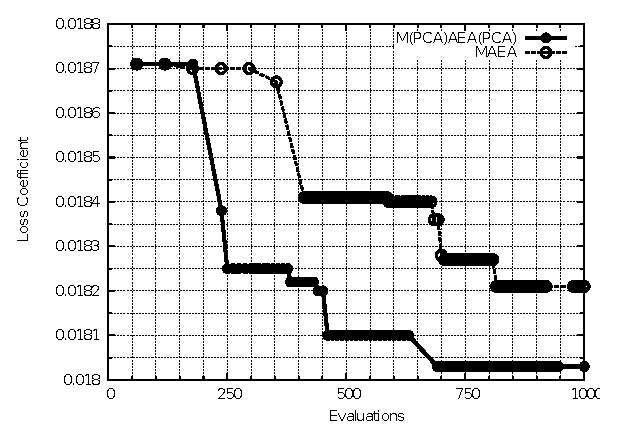
\includegraphics{CompPCA.eps}}
\end{minipage}
\caption{Σχεδιασμός 2Δ πτερύγωσης συμπιεστή: Πορείες σύγκλισης για ΜΑΕΑ και  Μ(\english{PCA})ΑΕΑ(\english{PCA}). Ως κριτήριο τερματισμού τέθηκε ο μέγιστος επιτρεπόμενος αριθμός αξιολογήσεων μέσω του λογισμικού ΥΡΔ (ίσος με 1000 κλήσεις).} 
\label{PCADrelaRes}
\end{figure}

Η βέλτιστη αεροτομή, όπως αυτή προέκυψε από το συνδυασμό των προτεινόμενων μεθόδων παρουσιάζεται στο σχήμα \ref{PCADrelaRes2} και έχει απώλειες $\omega\!=\!0.01803$ και στροφή της ροής $\Delta a\!=\!30^o$ ενώ, παράλληλα, ικανοποιεί και όλους τους γεωμετρικούς περιορισμούς.  

\begin{figure}[h!]
\begin{minipage}[b]{1\linewidth}
 \centering
 \resizebox*{14cm}{!}{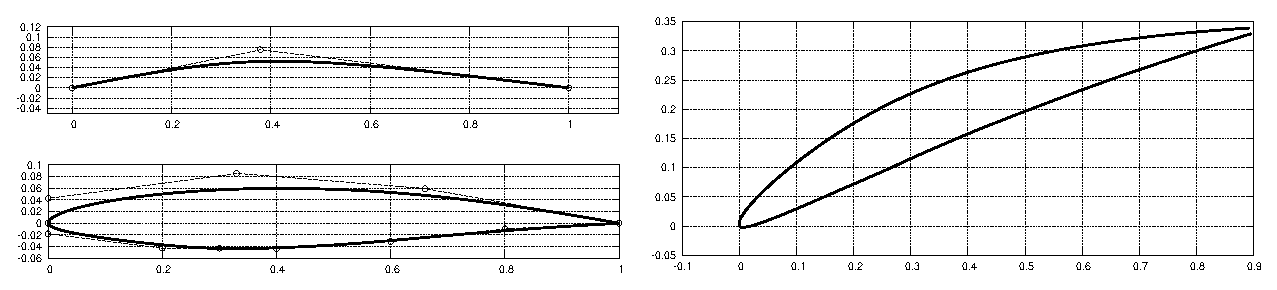
\includegraphics{ResD.eps}}
\end{minipage}
\caption{Σχεδιασμός 2Δ πτερύγωσης συμπιεστή: Η βέλτιστη αεροτομή, όπως αυτή σχεδιάστηκε από τον Μ(\english{PCA})ΑΕΑ(\english{PCA}). Αριστερά: Η μέση γραμμή και οι κατανομές πάχους για τις πλευρές υπερπίεσης και υποπίεσης, μαζί με τα πολύγωνα ελέγχου των πολυωνύμων \english{NURBS} που τις παρήγαγαν. Δεξιά: Η βέλτιστη αεροτομή, τοποθετημένη στην επιθυμητή γωνία κλίσης της πτερύγωσης. Η αεροτομή ικανοποιεί όλους τους τεθέντες περιορισμούς.} 
\label{PCADrelaRes2}
\end{figure}

%\begin{figure}[h!]
%\begin{minipage}[b]{1\linewidth}
% \centering
% \resizebox*{12cm}{!}{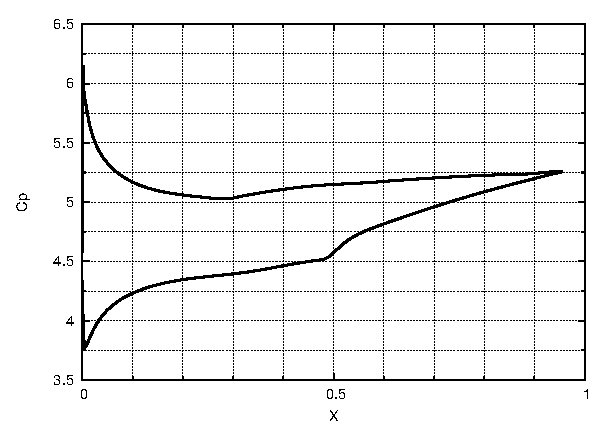
\includegraphics{Best_CP_PCA.eps}}
%\end{minipage}
%\caption{Σχεδιασμός 2Δ πτέρυγωσης συμπιεστή: Συντελεστής πίεσης $C_p$ για την βέλτιστη αεροτομή της εικόνας \ref{PCADrelaRes2}.} 
%\label{PCADrelaRes_cp}
%\end{figure}

% ---------------------------------------------------------------------------
% ----------------------- end of thesis sub-document ------------------------
% ---------------------------------------------------------------------------